\documentclass{extbook}[14pt]
\usepackage{multicol, enumerate, enumitem, hyperref, color, soul, setspace, parskip, fancyhdr, amssymb, amsthm, amsmath, latexsym, units, mathtools}
\everymath{\displaystyle}
\usepackage[headsep=0.5cm,headheight=0cm, left=1 in,right= 1 in,top= 1 in,bottom= 1 in]{geometry}
\usepackage{dashrule}  % Package to use the command below to create lines between items
\newcommand{\litem}[1]{\item #1

\rule{\textwidth}{0.4pt}}
\pagestyle{fancy}
\lhead{}
\chead{Answer Key for Progress Quiz 5 Version B}
\rhead{}
\lfoot{8497-6012}
\cfoot{}
\rfoot{Summer C 2021}
\begin{document}
\textbf{This key should allow you to understand why you choose the option you did (beyond just getting a question right or wrong). \href{https://xronos.clas.ufl.edu/mac1105spring2020/courseDescriptionAndMisc/Exams/LearningFromResults}{More instructions on how to use this key can be found here}.}

\textbf{If you have a suggestion to make the keys better, \href{https://forms.gle/CZkbZmPbC9XALEE88}{please fill out the short survey here}.}

\textit{Note: This key is auto-generated and may contain issues and/or errors. The keys are reviewed after each exam to ensure grading is done accurately. If there are issues (like duplicate options), they are noted in the offline gradebook. The keys are a work-in-progress to give students as many resources to improve as possible.}

\rule{\textwidth}{0.4pt}

\begin{enumerate}\litem{
Construct the lowest-degree polynomial given the zeros below. Then, choose the intervals that contain the coefficients of the polynomial in the form $x^3+bx^2+cx+d$.
\[ -5 + 4 i \text{ and } 1 \]The solution is \( x^{3} +9 x^{2} +31 x -41 \), which is option A.\begin{enumerate}[label=\Alph*.]
\item \( b \in [7, 12], c \in [31, 38], \text{ and } d \in [-48, -38] \)

* $x^{3} +9 x^{2} +31 x -41$, which is the correct option.
\item \( b \in [0, 5], c \in [-2, 10], \text{ and } d \in [-10, -2] \)

$x^{3} + x^{2} +4 x -5$, which corresponds to multiplying out $(x + 5)(x -1)$.
\item \( b \in [-10, -7], c \in [31, 38], \text{ and } d \in [35, 42] \)

$x^{3} -9 x^{2} +31 x + 41$, which corresponds to multiplying out $(x-(-5 + 4 i))(x-(-5 - 4 i))(x + 1)$.
\item \( b \in [0, 5], c \in [-7, 0], \text{ and } d \in [2, 5] \)

$x^{3} + x^{2} -5 x + 4$, which corresponds to multiplying out $(x -4)(x -1)$.
\item \( \text{None of the above.} \)

This corresponds to making an unanticipated error or not understanding how to use nonreal complex numbers to create the lowest-degree polynomial. If you chose this and are not sure what you did wrong, please contact the coordinator for help.
\end{enumerate}

\textbf{General Comment:} Remember that the conjugate of $a+bi$ is $a-bi$. Since these zeros always come in pairs, we need to multiply out $(x-(-5 + 4 i))(x-(-5 - 4 i))(x-(1))$.
}
\litem{
Construct the lowest-degree polynomial given the zeros below. Then, choose the intervals that contain the coefficients of the polynomial in the form $ax^3+bx^2+cx+d$.
\[ \frac{-7}{3}, \frac{-3}{2}, \text{ and } -1 \]The solution is \( 6x^{3} +29 x^{2} +44 x + 21 \), which is option E.\begin{enumerate}[label=\Alph*.]
\item \( a \in [0, 8], b \in [-18, -13], c \in [-7, -1], \text{ and } d \in [20, 27] \)

$6x^{3} -17 x^{2} -2 x + 21$, which corresponds to multiplying out $(3x -7)(2x -3)(x + 1)$.
\item \( a \in [0, 8], b \in [-31, -26], c \in [43, 48], \text{ and } d \in [-21, -18] \)

$6x^{3} -29 x^{2} +44 x -21$, which corresponds to multiplying out $(3x -7)(2x -3)(x -1)$.
\item \( a \in [0, 8], b \in [-2, 12], c \in [-29, -22], \text{ and } d \in [-21, -18] \)

$6x^{3} + x^{2} -26 x -21$, which corresponds to multiplying out $(3x -7)(2x + 3)(x + 1)$.
\item \( a \in [0, 8], b \in [26, 34], c \in [43, 48], \text{ and } d \in [-21, -18] \)

$6x^{3} +29 x^{2} +44 x -21$, which corresponds to multiplying everything correctly except the constant term.
\item \( a \in [0, 8], b \in [26, 34], c \in [43, 48], \text{ and } d \in [20, 27] \)

* $6x^{3} +29 x^{2} +44 x + 21$, which is the correct option.
\end{enumerate}

\textbf{General Comment:} To construct the lowest-degree polynomial, you want to multiply out $(3x + 7)(2x + 3)(x + 1)$
}
\litem{
Describe the end behavior of the polynomial below.
\[ f(x) = 8(x + 3)^{5}(x - 3)^{10}(x + 9)^{2}(x - 9)^{3} \]The solution is the graph below, which is option C.
    \begin{center}
        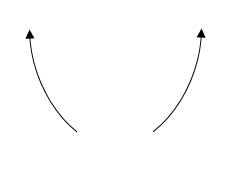
\includegraphics[width=0.3\textwidth]{../Figures/polyEndBehaviorCB.png}
    \end{center}\begin{enumerate}[label=\Alph*.]
\begin{multicols}{2}
\item 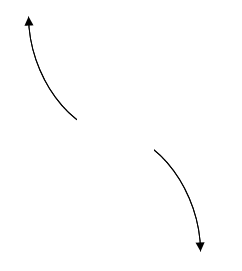
\includegraphics[width = 0.3\textwidth]{../Figures/polyEndBehaviorAB.png}
\item 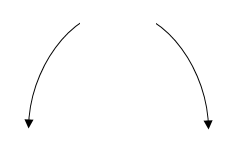
\includegraphics[width = 0.3\textwidth]{../Figures/polyEndBehaviorBB.png}
\item 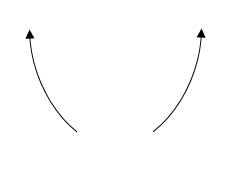
\includegraphics[width = 0.3\textwidth]{../Figures/polyEndBehaviorCB.png}
\item 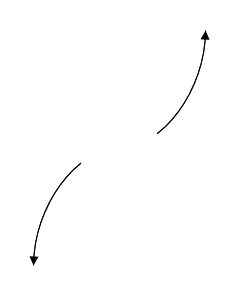
\includegraphics[width = 0.3\textwidth]{../Figures/polyEndBehaviorDB.png}
\end{multicols}\item None of the above.\end{enumerate}
\textbf{General Comment:} Remember that end behavior is determined by the leading coefficient AND whether the \textbf{sum} of the multiplicities is positive or negative.
}
\litem{
Which of the following equations \textit{could} be of the graph presented below?

\begin{center}
    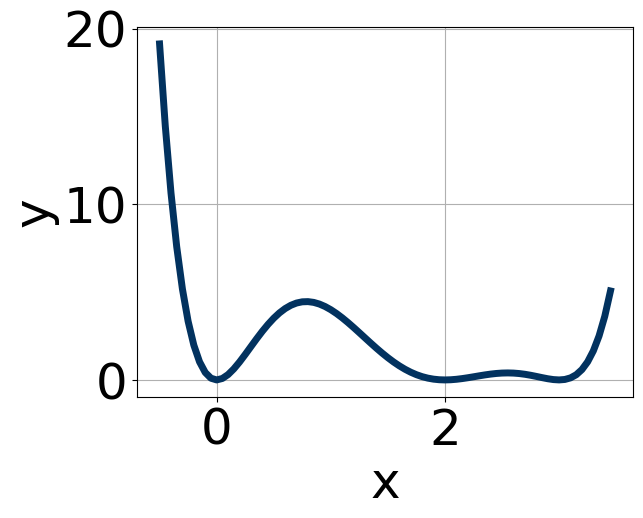
\includegraphics[width=0.5\textwidth]{../Figures/polyGraphToFunctionCopyB.png}
\end{center}


The solution is \( 20x^{8} (x - 3)^{4} (x - 2)^{6} \), which is option C.\begin{enumerate}[label=\Alph*.]
\item \( -6x^{10} (x - 3)^{8} (x - 2)^{11} \)

The factor $(x - 2)$ should have an even power and the leading coefficient should be the opposite sign.
\item \( -12x^{8} (x - 3)^{10} (x - 2)^{10} \)

This corresponds to the leading coefficient being the opposite value than it should be.
\item \( 20x^{8} (x - 3)^{4} (x - 2)^{6} \)

* This is the correct option.
\item \( 19x^{10} (x - 3)^{10} (x - 2)^{5} \)

The factor $(x - 2)$ should have an even power.
\item \( 17x^{7} (x - 3)^{8} (x - 2)^{7} \)

The factors $x$ and $(x - 2)$ should both have even powers.
\end{enumerate}

\textbf{General Comment:} General Comments: Draw the x-axis to determine which zeros are touching (and so have even multiplicity) or cross (and have odd multiplicity).
}
\litem{
Construct the lowest-degree polynomial given the zeros below. Then, choose the intervals that contain the coefficients of the polynomial in the form $ax^3+bx^2+cx+d$.
\[ \frac{-3}{4}, 4, \text{ and } \frac{4}{3} \]The solution is \( 12x^{3} -55 x^{2} +16 x + 48 \), which is option C.\begin{enumerate}[label=\Alph*.]
\item \( a \in [6, 19], b \in [54, 56], c \in [13, 20], \text{ and } d \in [-52, -44] \)

$12x^{3} +55 x^{2} +16 x -48$, which corresponds to multiplying out $(4x -3)(x + 4)(3x + 4)$.
\item \( a \in [6, 19], b \in [-58, -53], c \in [13, 20], \text{ and } d \in [-52, -44] \)

$12x^{3} -55 x^{2} +16 x -48$, which corresponds to multiplying everything correctly except the constant term.
\item \( a \in [6, 19], b \in [-58, -53], c \in [13, 20], \text{ and } d \in [47, 52] \)

* $12x^{3} -55 x^{2} +16 x + 48$, which is the correct option.
\item \( a \in [6, 19], b \in [22, 29], c \in [-90, -84], \text{ and } d \in [47, 52] \)

$12x^{3} +23 x^{2} -88 x + 48$, which corresponds to multiplying out $(4x -3)(x + 4)(3x -4)$.
\item \( a \in [6, 19], b \in [-77, -65], c \in [111, 121], \text{ and } d \in [-52, -44] \)

$12x^{3} -73 x^{2} +112 x -48$, which corresponds to multiplying out $(4x -3)(x -4)(3x -4)$.
\end{enumerate}

\textbf{General Comment:} To construct the lowest-degree polynomial, you want to multiply out $(4x + 3)(x -4)(3x -4)$
}
\litem{
Which of the following equations \textit{could} be of the graph presented below?

\begin{center}
    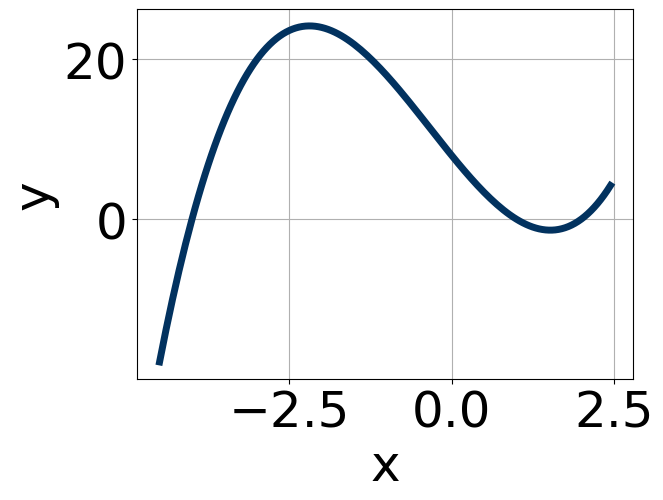
\includegraphics[width=0.5\textwidth]{../Figures/polyGraphToFunctionB.png}
\end{center}


The solution is \( 11(x - 1)^{7} (x - 2)^{9} (x + 4)^{7} \), which is option C.\begin{enumerate}[label=\Alph*.]
\item \( -7(x - 1)^{8} (x - 2)^{7} (x + 4)^{11} \)

The factor $(x - 1)$ should have an odd power and the leading coefficient should be the opposite sign.
\item \( -17(x - 1)^{5} (x - 2)^{9} (x + 4)^{9} \)

This corresponds to the leading coefficient being the opposite value than it should be.
\item \( 11(x - 1)^{7} (x - 2)^{9} (x + 4)^{7} \)

* This is the correct option.
\item \( 20(x - 1)^{10} (x - 2)^{8} (x + 4)^{11} \)

The factors $1$ and $2$ have have been odd power.
\item \( 18(x - 1)^{6} (x - 2)^{11} (x + 4)^{5} \)

The factor $1$ should have been an odd power.
\end{enumerate}

\textbf{General Comment:} General Comments: Draw the x-axis to determine which zeros are touching (and so have even multiplicity) or cross (and have odd multiplicity).
}
\litem{
Describe the zero behavior of the zero $x = -4$ of the polynomial below.
\[ f(x) = 4(x + 4)^{8}(x - 4)^{13}(x - 8)^{2}(x + 8)^{6} \]The solution is the graph below, which is option B.
    \begin{center}
        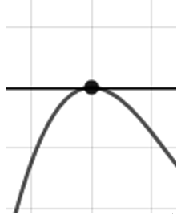
\includegraphics[width=0.3\textwidth]{../Figures/polyZeroBehaviorBB.png}
    \end{center}\begin{enumerate}[label=\Alph*.]
\begin{multicols}{2}
\item 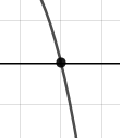
\includegraphics[width = 0.3\textwidth]{../Figures/polyZeroBehaviorAB.png}
\item 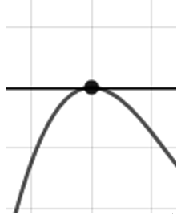
\includegraphics[width = 0.3\textwidth]{../Figures/polyZeroBehaviorBB.png}
\item 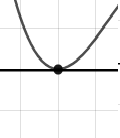
\includegraphics[width = 0.3\textwidth]{../Figures/polyZeroBehaviorCB.png}
\item 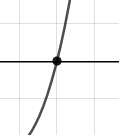
\includegraphics[width = 0.3\textwidth]{../Figures/polyZeroBehaviorDB.png}
\end{multicols}\item None of the above.\end{enumerate}
\textbf{General Comment:} You will need to sketch the entire graph, then zoom in on the zero the question asks about.
}
\litem{
Describe the zero behavior of the zero $x = -6$ of the polynomial below.
\[ f(x) = -4(x - 8)^{12}(x + 8)^{8}(x + 6)^{11}(x - 6)^{8} \]The solution is the graph below, which is option A.
    \begin{center}
        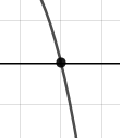
\includegraphics[width=0.3\textwidth]{../Figures/polyZeroBehaviorCopyAB.png}
    \end{center}\begin{enumerate}[label=\Alph*.]
\begin{multicols}{2}
\item 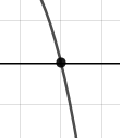
\includegraphics[width = 0.3\textwidth]{../Figures/polyZeroBehaviorCopyAB.png}
\item 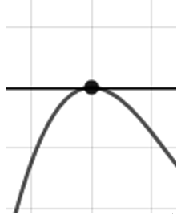
\includegraphics[width = 0.3\textwidth]{../Figures/polyZeroBehaviorCopyBB.png}
\item 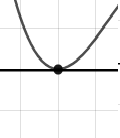
\includegraphics[width = 0.3\textwidth]{../Figures/polyZeroBehaviorCopyCB.png}
\item 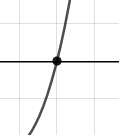
\includegraphics[width = 0.3\textwidth]{../Figures/polyZeroBehaviorCopyDB.png}
\end{multicols}\item None of the above.\end{enumerate}
\textbf{General Comment:} You will need to sketch the entire graph, then zoom in on the zero the question asks about.
}
\litem{
Construct the lowest-degree polynomial given the zeros below. Then, choose the intervals that contain the coefficients of the polynomial in the form $x^3+bx^2+cx+d$.
\[ -5 + 4 i \text{ and } 4 \]The solution is \( x^{3} +6 x^{2} +x -164 \), which is option D.\begin{enumerate}[label=\Alph*.]
\item \( b \in [-7.2, -3.1], c \in [-6, 9], \text{ and } d \in [157, 173] \)

$x^{3} -6 x^{2} +x + 164$, which corresponds to multiplying out $(x-(-5 + 4 i))(x-(-5 - 4 i))(x + 4)$.
\item \( b \in [-1.8, 4.3], c \in [-6, 9], \text{ and } d \in [-26, -16] \)

$x^{3} + x^{2} +x -20$, which corresponds to multiplying out $(x + 5)(x -4)$.
\item \( b \in [-1.8, 4.3], c \in [-10, -5], \text{ and } d \in [16, 23] \)

$x^{3} + x^{2} -8 x + 16$, which corresponds to multiplying out $(x -4)(x -4)$.
\item \( b \in [5.4, 7.5], c \in [-6, 9], \text{ and } d \in [-165, -163] \)

* $x^{3} +6 x^{2} +x -164$, which is the correct option.
\item \( \text{None of the above.} \)

This corresponds to making an unanticipated error or not understanding how to use nonreal complex numbers to create the lowest-degree polynomial. If you chose this and are not sure what you did wrong, please contact the coordinator for help.
\end{enumerate}

\textbf{General Comment:} Remember that the conjugate of $a+bi$ is $a-bi$. Since these zeros always come in pairs, we need to multiply out $(x-(-5 + 4 i))(x-(-5 - 4 i))(x-(4))$.
}
\litem{
Describe the end behavior of the polynomial below.
\[ f(x) = 4(x - 9)^{3}(x + 9)^{8}(x - 8)^{4}(x + 8)^{4} \]The solution is the graph below, which is option D.
    \begin{center}
        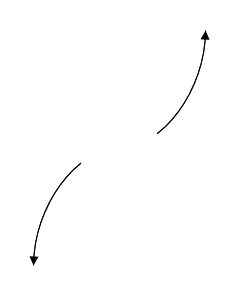
\includegraphics[width=0.3\textwidth]{../Figures/polyEndBehaviorCopyDB.png}
    \end{center}\begin{enumerate}[label=\Alph*.]
\begin{multicols}{2}
\item 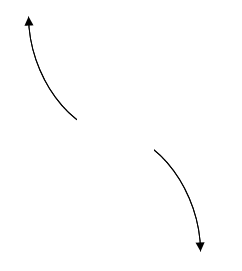
\includegraphics[width = 0.3\textwidth]{../Figures/polyEndBehaviorCopyAB.png}
\item 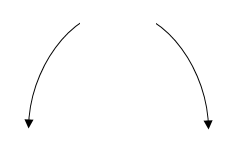
\includegraphics[width = 0.3\textwidth]{../Figures/polyEndBehaviorCopyBB.png}
\item 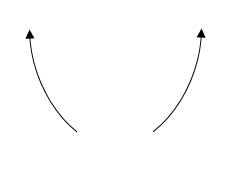
\includegraphics[width = 0.3\textwidth]{../Figures/polyEndBehaviorCopyCB.png}
\item 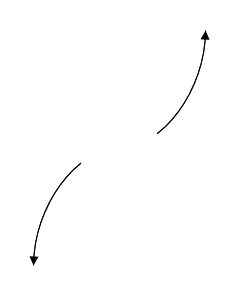
\includegraphics[width = 0.3\textwidth]{../Figures/polyEndBehaviorCopyDB.png}
\end{multicols}\item None of the above.\end{enumerate}
\textbf{General Comment:} Remember that end behavior is determined by the leading coefficient AND whether the \textbf{sum} of the multiplicities is positive or negative.
}
\end{enumerate}

\end{document}